\documentclass[zavrsnirad]{fer}

\usepackage{blindtext}

\title{Key distribution and secure updates on Internet of things devices}
\naslov{Distribucija ključeva i sigurnosnih ažuriranja na uređajima Interneta stvari}
\brojrada{1234} % Thesis number
\author{Roko Gligora}
\mentor{Prof.\@ Marin Vuković}
\date{June, 2024}
\datum{lipanj, 2024.}


\begin{document}
	\maketitle
	
	Uređaji Interneta stvari zbog tipično lošije povezivosti, slabije memorijske i procesorske snage, kao i ograničenog napajanja često zaostaju za tradicionalnim uređajima u smislu sigurnih ažuriranja i sigurnosti općenito. Jedan od ključnih aspekata bilo kojeg uređaja koji komunicira jest razmjena kriptografskih ključeva te provođenje ažuriranja na siguran način.
	
	Vaš je zadatak analizirati postojeća rješenja za navedene izazove u domeni Interneta stvari. Na temelju analize osmislite i implementirajte sustav za upravljanje ključevima te efikasno i sigurno ažuriranje. Obratite pozornost na procjenu opterećenja uređaja prilikom ažuriranja i postavljanja ključeva kako se ne bi narušile osnovne funkcionalnosti uređaja prilikom navedenih radnji.
	
	\begin{zahvale}
		acknowledgment
	\end{zahvale}
	
	\mainmatter
	
	\tableofcontents
	
	\chapter{Uvod}
	\label{pog:uvod}
	
	Neki od radova koje ćemo citirati su \cite{maurer1993secret}.
	Trebaju nam samo radi testiranja kako izgleda referenciranje rada s konferencije, rada iz časopisa, knjige i Internetske stranice.
	
	\begin{figure}[htb]
		\centering
		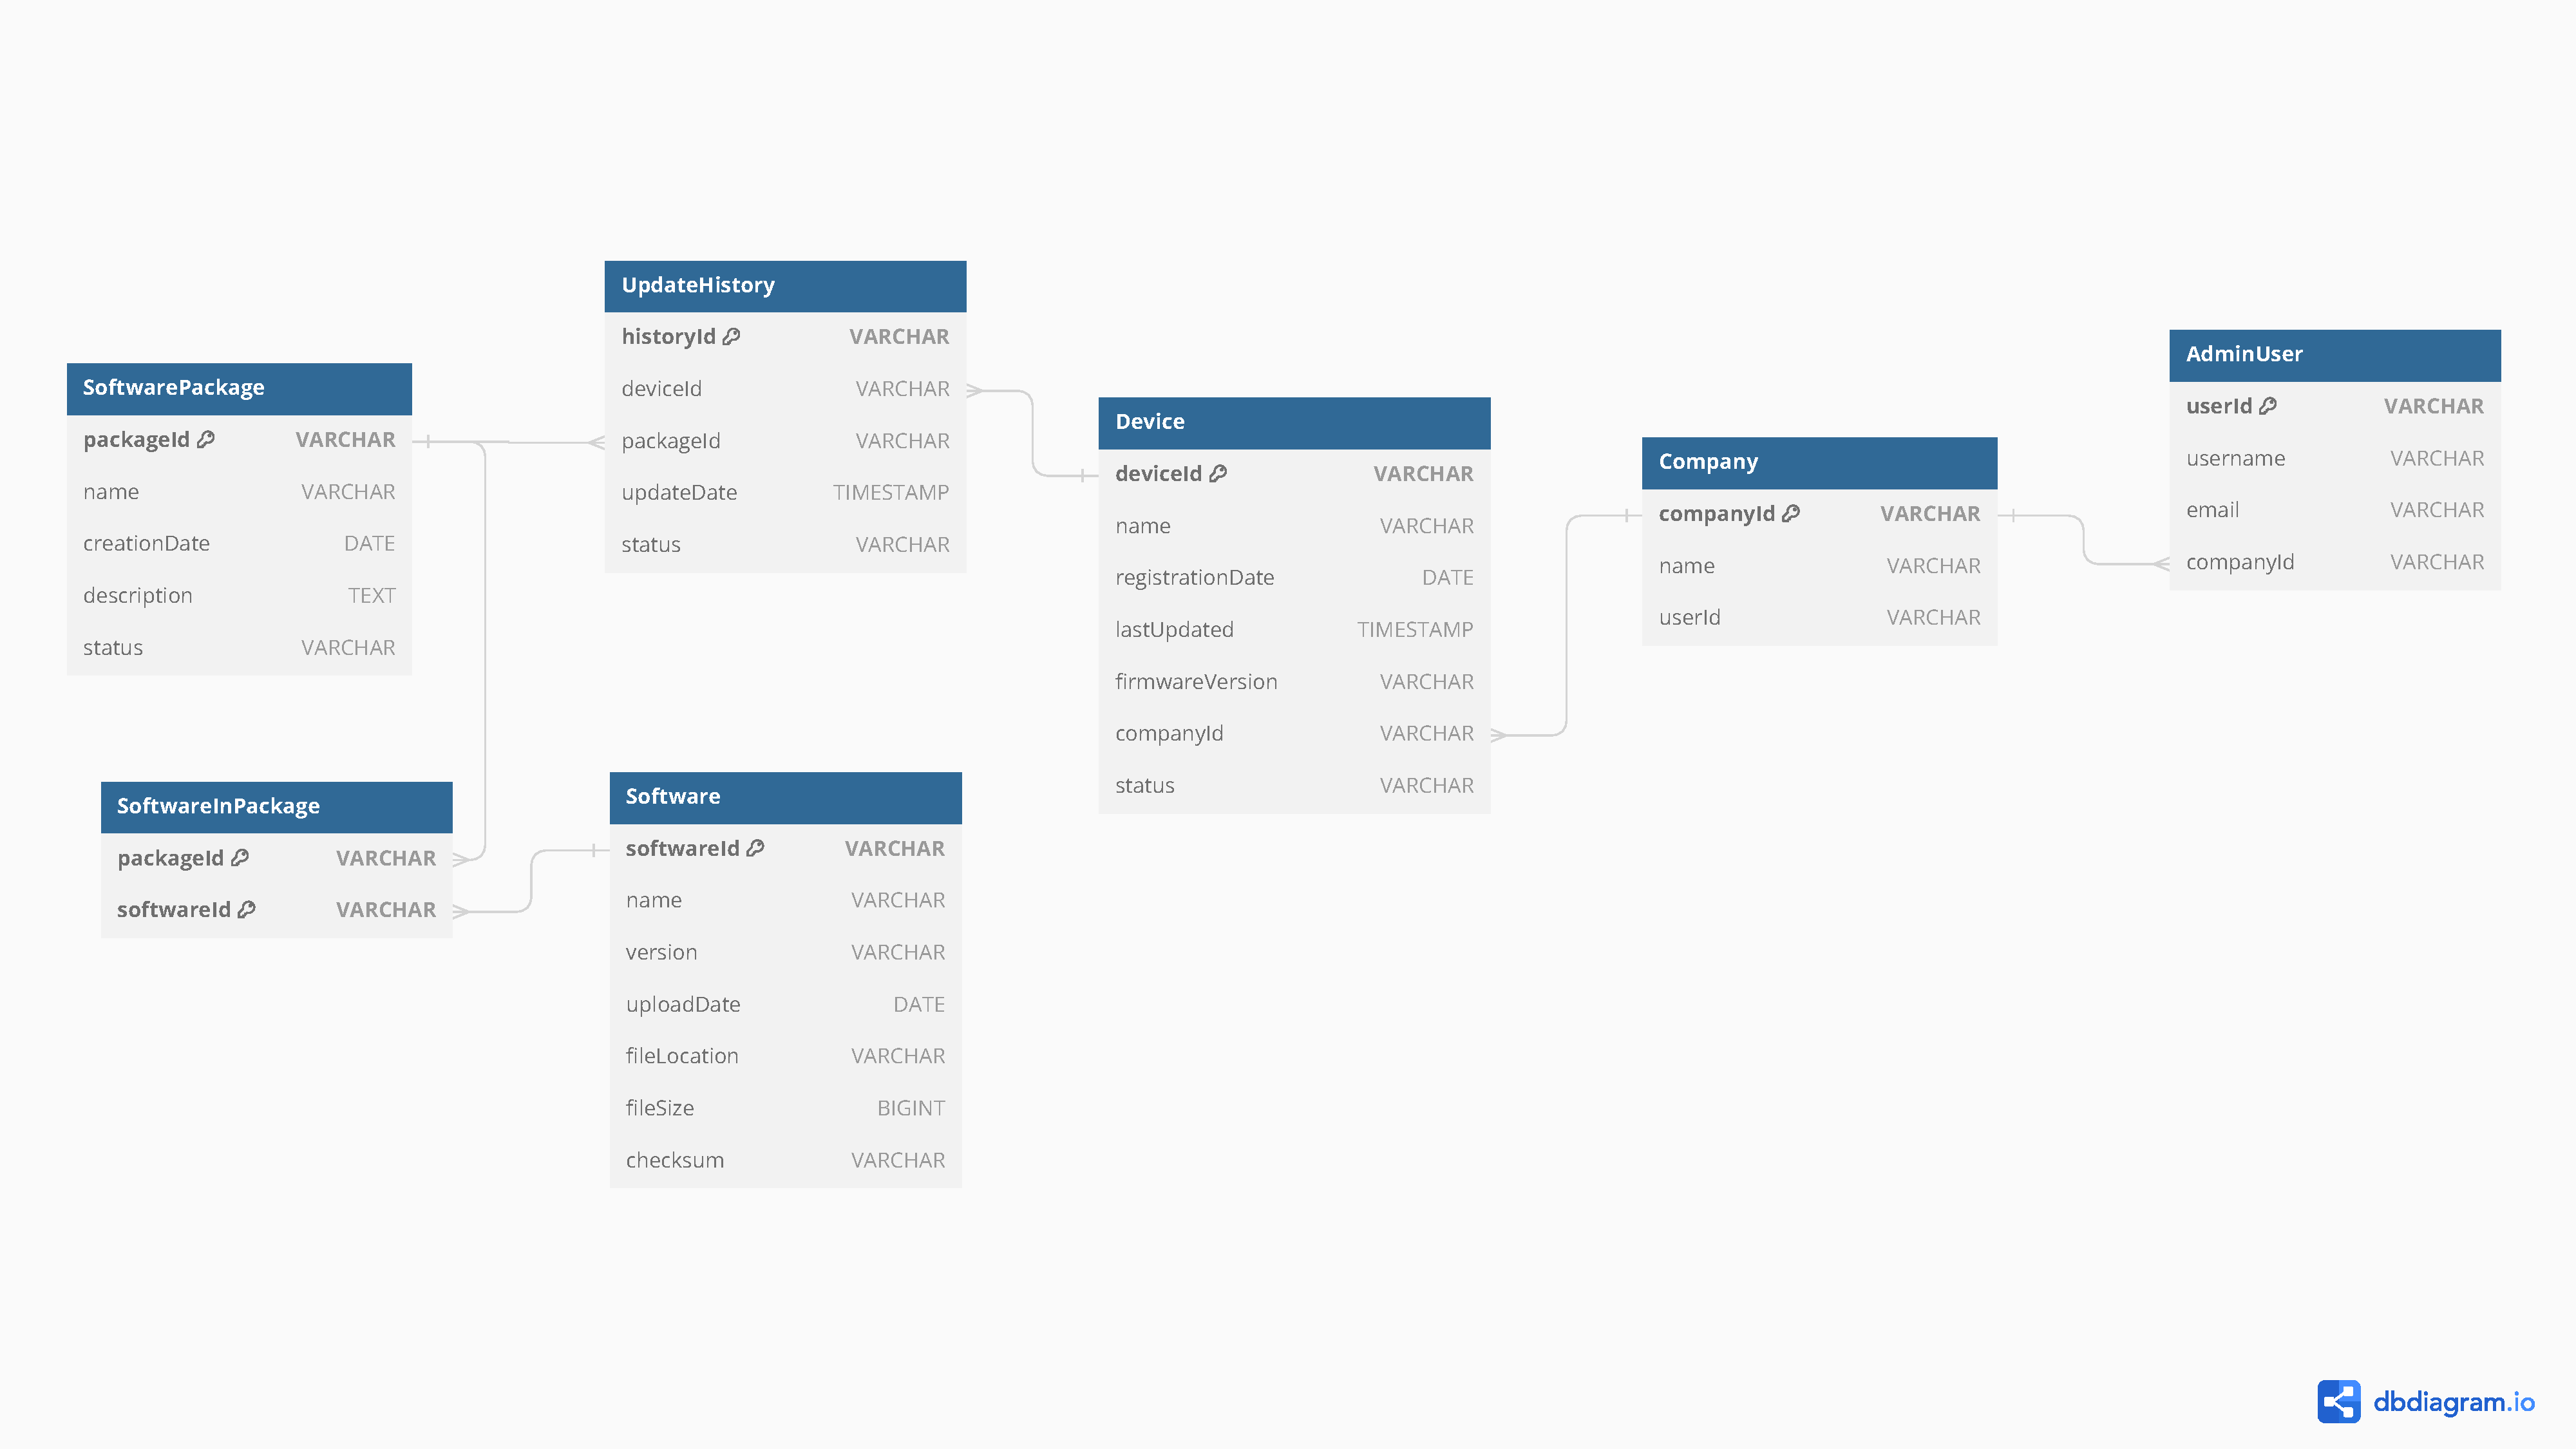
\includegraphics[width=0.38\linewidth]{Figures/ER_diagram_KDSUF_v2.pdf} 
		\caption{Moja prva slika}
		\label{slk:prvaslika}
	\end{figure}
	
	Referenciramo se na sliku \ref{slk:prvaslika} u sredini rečenice, zatim prije zareza \ref{slk:prvaslika}, te zatim na kraju rečenice \ref{slk:prvaslika}.
	Upravo smo testirali radi li naredba \verb|\ref| ispravno u slučaju kada nakon nje slijedi točka.
	
	
	
	%-------------------------------------------------------------------------------
	\chapter{Glavni dio}
	\label{pog:glavni_dio}
	
	\Blindtext
	
	
	%-------------------------------------------------------------------------------
	\chapter{Rezultati i rasprava}
	\label{pog:rezultati_i_rasprava}
	
	\Blindtext
	
	
	%--- ZAKLJUČAK / CONCLUSION ----------------------------------------------------
	\chapter{Zaključak}
	\label{pog:zakljucak}
	
	\blindtext
	
	
	\bibliography{references}
	
		\begin{sazetak}
		sažetak na hrvatskom
	\end{sazetak}
	
	\begin{kljucnerijeci}
		ključne riječi na hrvatskom
	\end{kljucnerijeci}    
	
	\begin{abstract}
		abstract in English
	\end{abstract}
	
	\begin{keywords}
		keywords in English
	\end{keywords}
	
	\backmatter
	
	\chapter{The Code}
	
	\Blindtext
	

\end{document}